\begin{figure*}[ht!]
\begin{center}% note that \centering uses less vspace...
\resizebox{2\columnwidth}{!}{%
\begin{tabular}{lllll}


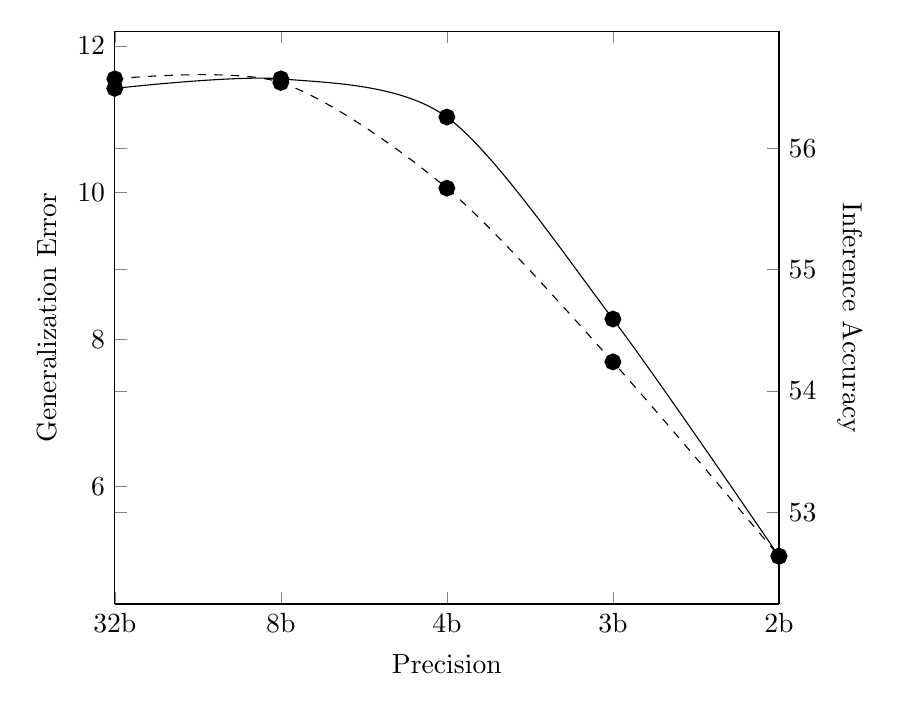
\begin{tikzpicture}
% let both axes use the same layers
\pgfplotsset{set layers}
%
\begin{axis}[
scale only axis,
line width=2.0pt,
mark size=2.0pt,
xmin=0,xmax=4,
ylabel={Generalization Error},
axis y line*=left,
xlabel={Precision},
xtick={0,1,2,3,4},
xticklabels={32b, 8b, 4b, 3b, 2b}
]
\addplot[
    color=black,
    solid,
    mark=*,
    mark options={solid},
    smooth
    ]
    coordinates {
    (0,11.42)(1,11.55)(2,11.03)(3,8.28)(4,5.05)
      };
\end{axis}

\begin{axis}[
scale only axis,
line width=2.0pt,
mark size=2.0pt,
xmin=0,xmax=4,
ylabel near ticks, yticklabel pos=right,
ylabel={Inference Accuracy},
ylabel style = {rotate=180},
axis x line=none
]
\addplot[
    color=black,
    dashed,
    mark=*,
    mark options={solid},
    smooth
    ]
    coordinates {
    (0,56.57)(1,56.54)(2,55.67)(3,54.24)(4,52.64)
        };
\end{axis}
\end{tikzpicture} &

%
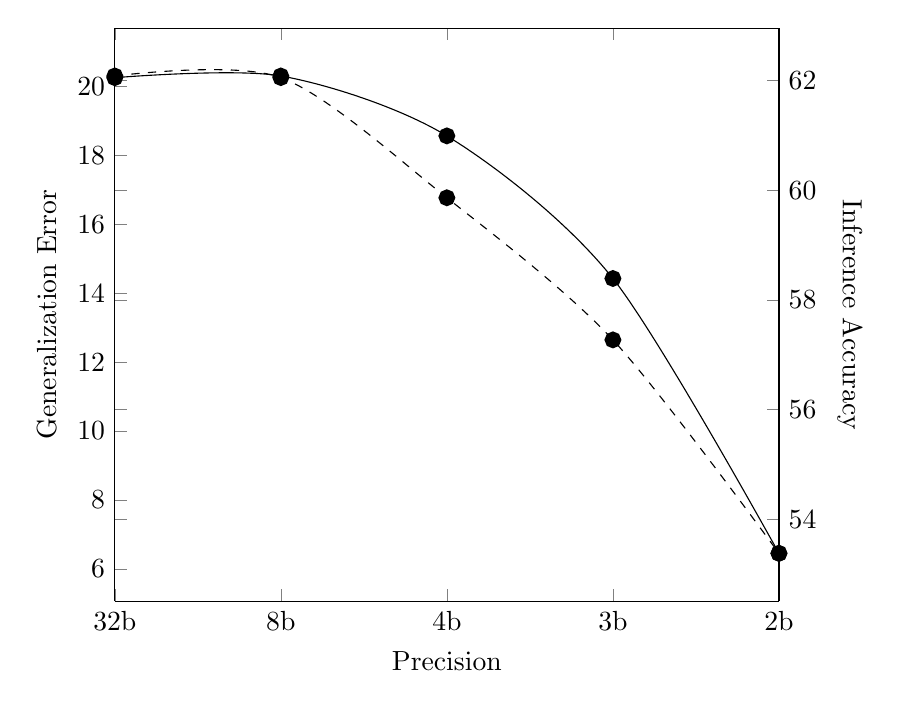
\begin{tikzpicture}
% let both axes use the same layers
\pgfplotsset{set layers}
%
\begin{axis}[
scale only axis,
line width=2.0pt,
mark size=2.0pt,
xmin=0,xmax=4,
ylabel={Generalization Error},
axis y line*=left,
xlabel={Precision},
xtick={0,1,2,3,4},
xticklabels={32b, 8b, 4b, 3b, 2b}
]
\addplot[
    color=black,
    solid,
    mark=*,
    mark options={solid},
    smooth
    ]
    coordinates {
    (0,20.26)(1,20.31)(2,18.57)(3,14.43)(4,6.45)
      };
\end{axis}

\begin{axis}[
scale only axis,
line width=2.0pt,
mark size=2.0pt,
xmin=0,xmax=4,
ylabel near ticks, yticklabel pos=right,
ylabel={Inference Accuracy},
ylabel style = {rotate=180},
axis x line=none
]
\addplot[
    color=black,
    dashed,
    mark=*,
    mark options={solid},
    smooth
    ]
    coordinates {
    (0,62.08)(1,62.05)(2,59.86)(3,57.27)(4,53.38)
        };
\end{axis}
\end{tikzpicture} &





%
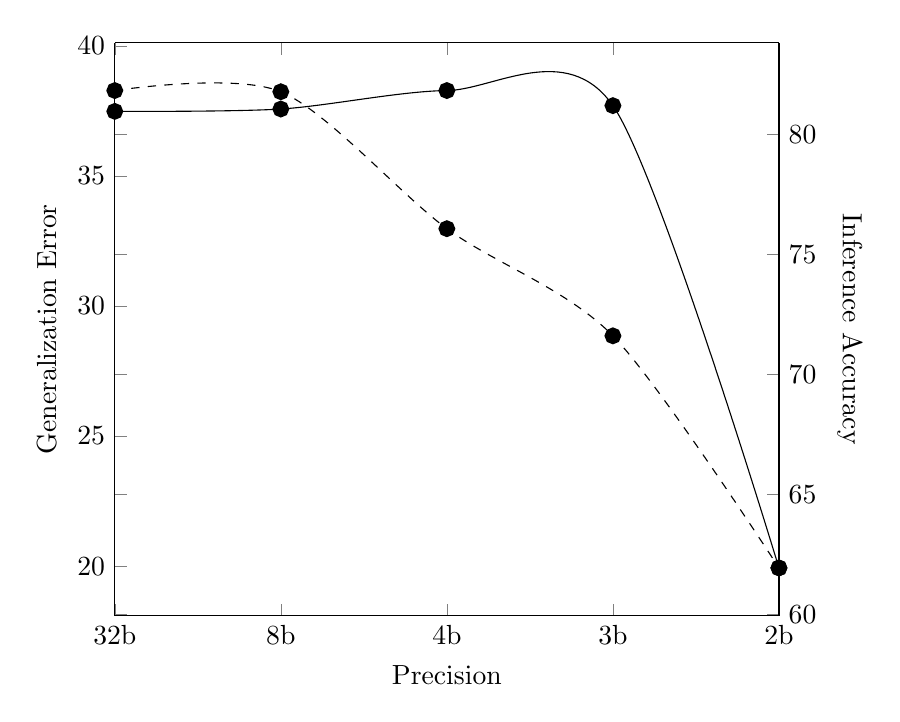
\begin{tikzpicture}
% let both axes use the same layers
\pgfplotsset{set layers}
%
\begin{axis}[
scale only axis,
line width=2.0pt,
mark size=2.0pt,
xmin=0,xmax=4,
ylabel={Generalization Error},
axis y line*=left,
xlabel={Precision},
xtick={0,1,2,3,4},
xticklabels={32b, 8b, 4b, 3b, 2b}
]
\addplot[
    color=black,
    solid,
    mark=*,
    mark options={solid},
    smooth
    ]
    coordinates {
    (0,37.48)(1,37.57)(2,38.28)(3,37.70)(4,19.93)
      };
\end{axis}

\begin{axis}[
scale only axis,
line width=2.0pt,
mark size=2.0pt,
xmin=0,xmax=4,
ylabel near ticks, yticklabel pos=right,
ylabel={Inference Accuracy},
ylabel style = {rotate=180},
axis x line=none
]
\addplot[
    color=black,
    dashed,
    mark=*,
    mark options={solid},
    smooth
    ]
    coordinates {
    (0,81.82)(1,81.77)(2,76.07)(3,71.61)(4,61.95)
        };
\end{axis}
\end{tikzpicture}


\end{tabular}
}
\caption{\underline{Pruning followed by Weight Sharing (Quantization).} While the retraining after pruning is necessary to restore the predictive accuracy, clustering the weights to reduce the precision lowers the inference accuracy (dashed line) risk while reducing the generalization error (solid line) for FashionMNIST(left), Purchase100(Center) and Location(Right) dataset.}
\label{fig:wtsharing}
\end{center}
\end{figure*}
